% Tento soubor nahraďte vlastním souborem s přílohami (nadpisy níže jsou pouze pro příklad)

% Pro kompilaci po částech (viz projekt.tex), nutno odkomentovat a upravit
%\documentclass[../projekt.tex]{subfiles}
%\begin{document}

% Umístění obsahu paměťového média do příloh je vhodné konzultovat s vedoucím
%\chapter{Obsah přiloženého paměťového média}

%\chapter{Manuál}

%\chapter{Konfigurační soubor}

%\chapter{RelaxNG Schéma konfiguračního souboru}

%\chapter{Plakát}

\chapter{Diagram tříd}

Tato příloha obsahuje diagram tříd, který reprezentuje strukturu programu. Jelikož je struktura programu velmi rozsáhlá, bylo nutné rozdělit diagram na několik částí.

První část obsahuje proces příchodu události (například stisku klávesy) z~knihovny SDL a~její následnou cestu ke kořenovému kontroleru. Nachází se zde také třída \uv{Main}, která představuje hlavní tělo programu.

Ve druhé části je znázorněn proces propagace události od kořenového kontroleru k~jeho \uv{dítěti}. Je zde znázorněno, jak bylo implementováno odebírání a~zahazování událostí v~jednotlivých nekořenových kontrolerech.

Ve třetí části je popsána třída, jež představuje rozhraní komunikaci s~SDL; obecně s~čímkoliv, co poskytuje přístup k~uživatelskému vstupu a~výstupu.

Diagram byl vytvořen pomocí nástroje \emph{draw.io} dostupného na \url{https://app.diagrams.net/}.

\todo{FIXME: Text odkazu přetéká \^\ }

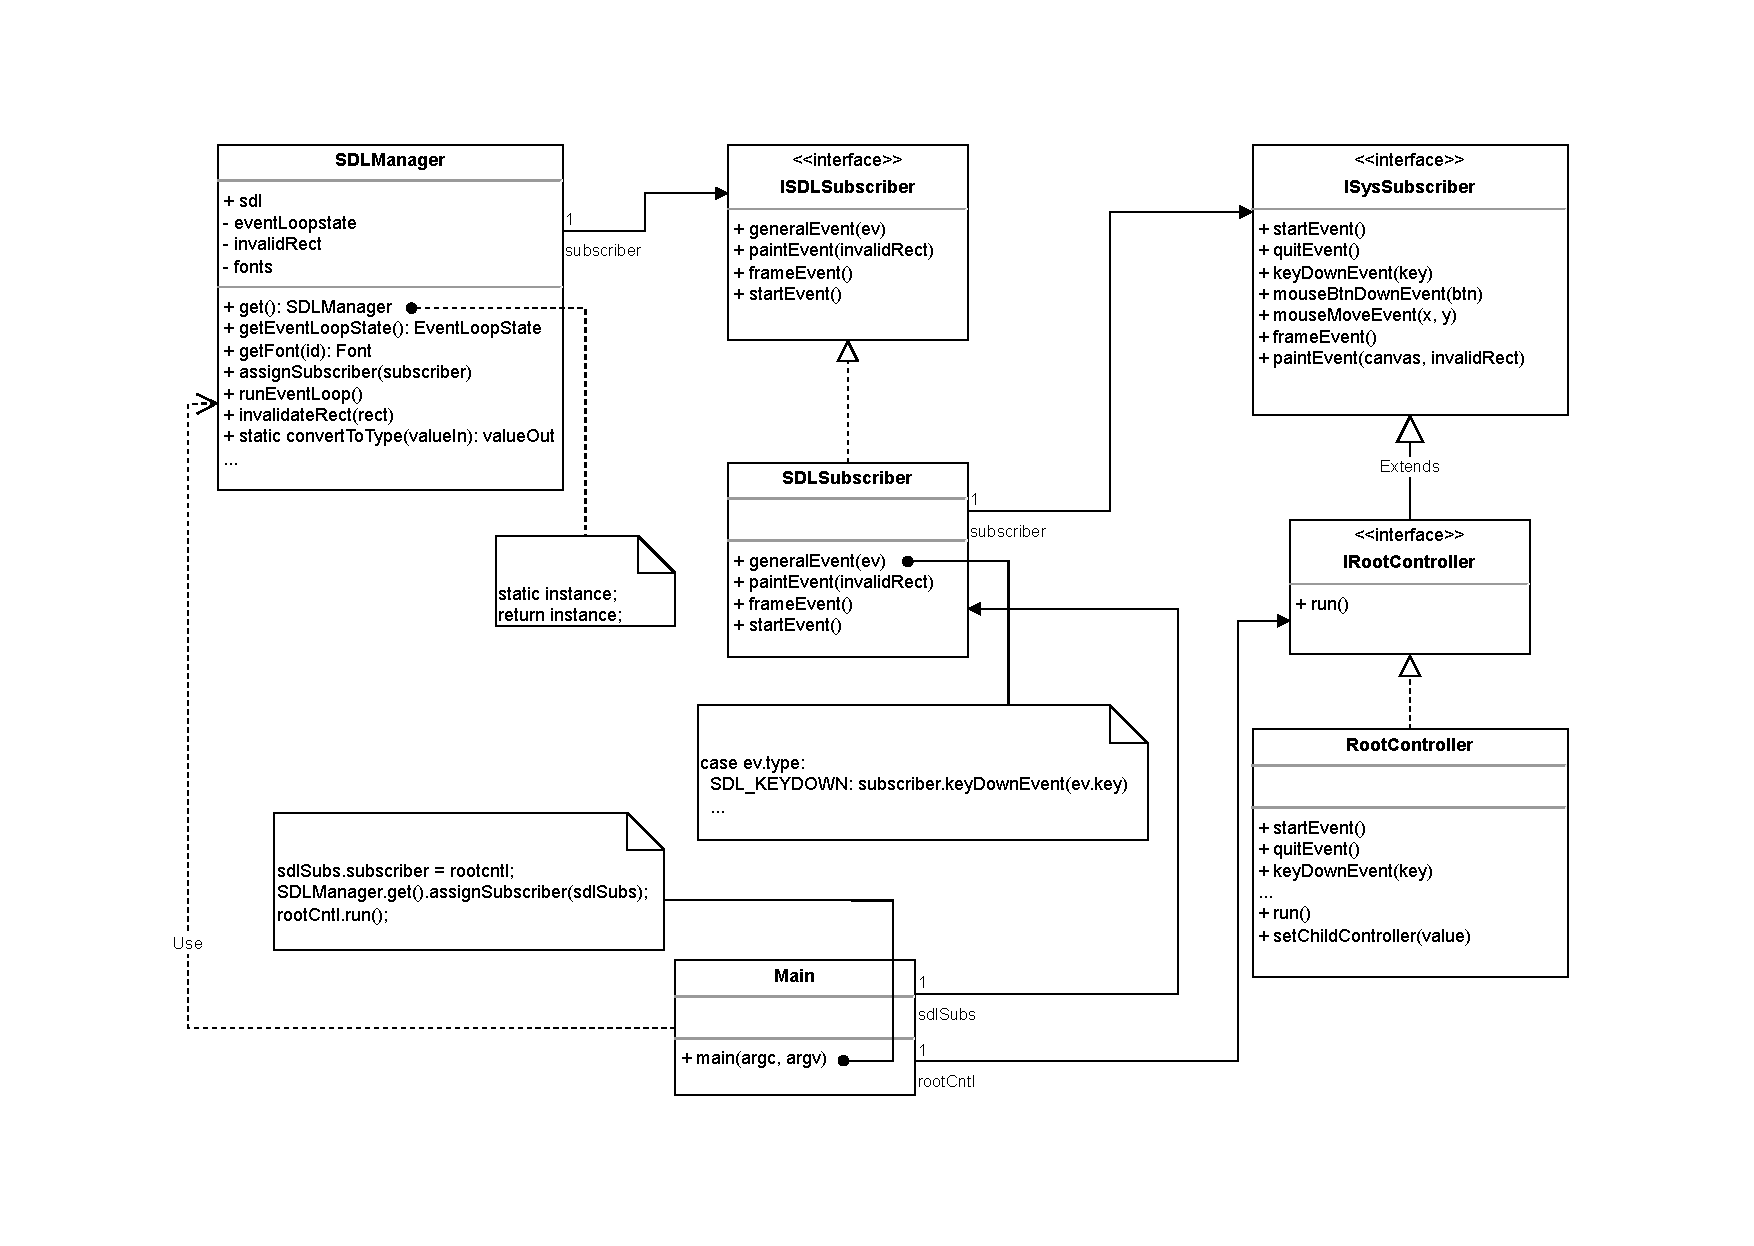
\includepdf[pages=-]{class-diagram.pdf}

% Pro kompilaci po částech (viz projekt.tex) nutno odkomentovat
%\end{document}
